\documentclass[11pt]{exam}
\usepackage[utf8]{inputenc}
\usepackage{hyperref}
\usepackage{graphicx}

\title{Clustering en Weka}
\author{Laura Rodríguez Navas \\ rodrigueznavas@posgrado.uimp.es}
\date{\today}

\pagestyle{plain}

\begin{document}
	
\maketitle

En esta práctica se realiza un estudio acerca de la base de datos Iris. Esta base de datos se distribuye junto a la herramienta \href{https://www.cs.waikato.ac.nz/ml/weka/}{Weka}.

\begin{questions}
	
% Pregunta 1
{\question Ejecuta el algoritmo SimpleKMeans usando la herramienta Weka con las distancias Euclídea y Manhattan.}

\renewcommand{\figurename}{Figura}

\begin{figure}[h]
	\centering
	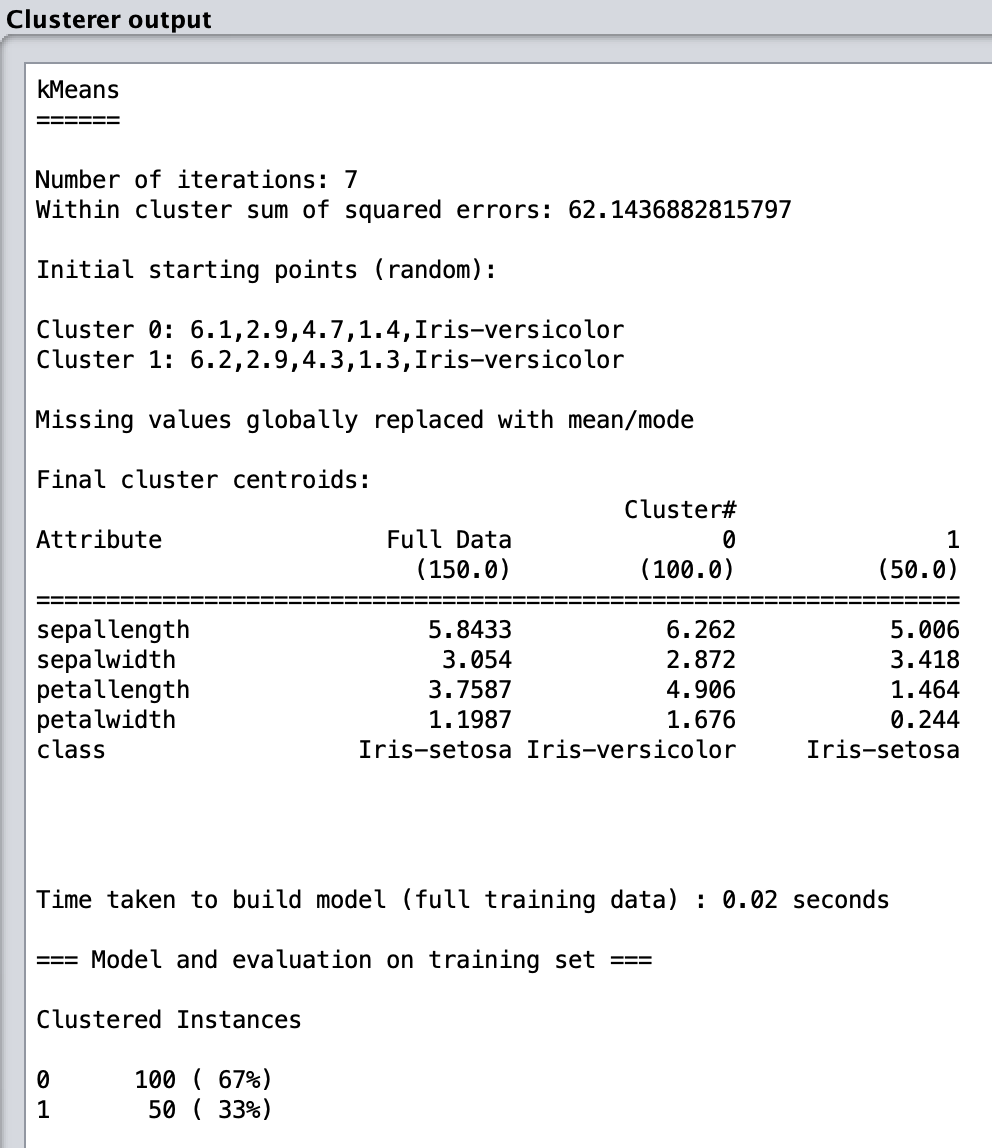
\includegraphics[scale=0.5]{kmeans_euclidea.png}
	\caption{KMeans con distancia Euclídea.}
	\label{Captura_1}
\end{figure}


\begin{figure}[h]
	\centering
	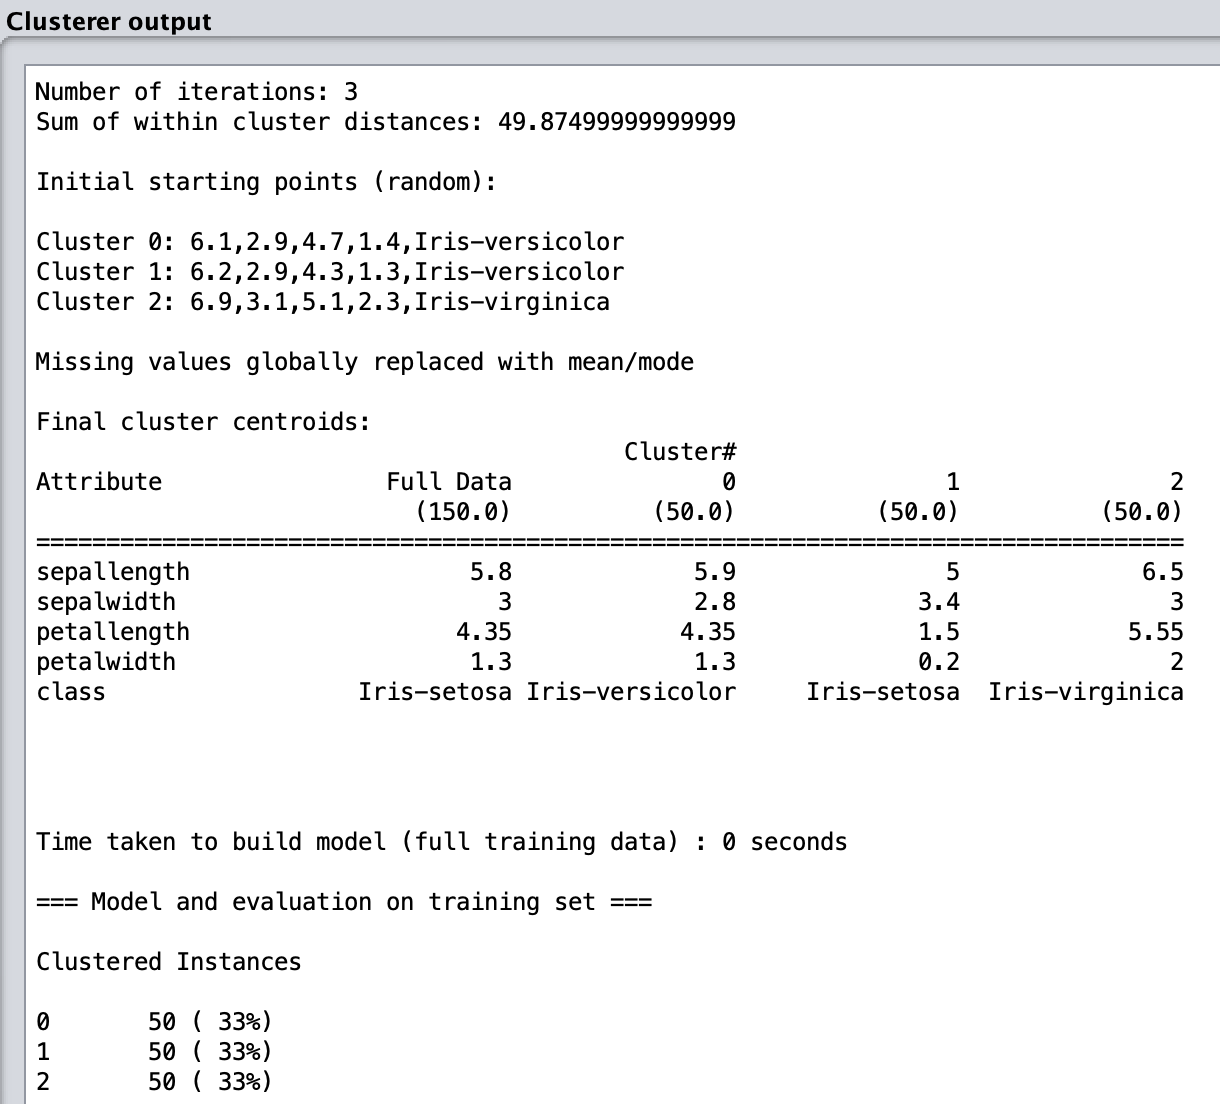
\includegraphics[scale=0.5]{kmeans_manhattan.png}
	\caption{KMeans con distancia Manhattan.}
	\label{Captura_2}
\end{figure}

\begin{parts}

\part ¿Cuántas instancias contiene cada grupo?

En la ejecución del algoritmo KMeans con distancia Euclídea (ver Figura \ref{Captura_1}) se han formado dos grupos: 0 y 1. El grupo 0 contienen 100 instancias (el 67\% de las instancias del conjunto de datos) y el grupo 1 contiene 50 instancias (el 33\% de las instancias del conjunto de datos). 

En la ejecución del algoritmo KMeans con distancia Manhattan (ver Figura \ref{Captura_2}) también se han formado los grupos 0 y 1. El grupo 0 contienen 98 instancias (el 65\% de las instancias del conjunto de datos) y el grupo 1 contiene 52 instancias (el 35\% de las instancias del conjunto de datos). 

\part ¿Cuáles son los centroides?

Si nos volvemos a fijar en la figura \ref{Captura_1}, podemos observar los centroides de la ejecución de Kmeans con distancia Euclídea. Se muestran en la siguiente figura:

\begin{figure}[h]
	\centering
	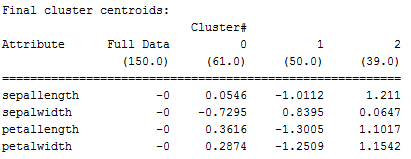
\includegraphics[scale=0.4]{kmeans_euclidea_centroides.png}
	\caption{KMeans centroides con distancia Euclídea.}
	\label{Captura_3}
\end{figure}

Y si nos volvemos a fijar en la figura \ref{Captura_2}, podemos observar los centroides de la ejecución de Kmeans con distancia Manhattan. Se muestran en la siguiente figura:

\begin{figure}[h]
	\centering
	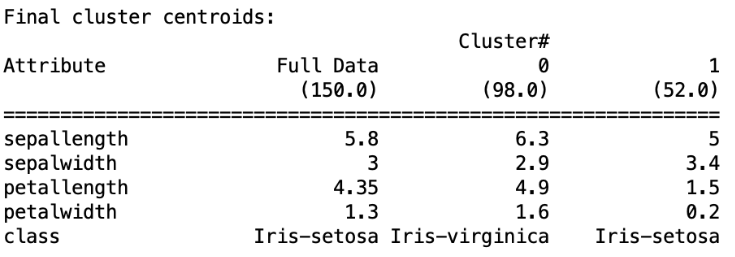
\includegraphics[scale=0.4]{kmeans_manhattan_centroides.png}
	\caption{KMeans centroides con distancia Manhattan.}
	\label{Captura_4}
\end{figure}

\part Analiza los centroides. ¿Hay algo destacable en esos centroides? ¿Están los centroides separados en el espacio? ¿Tienen componentes similares?

\end{parts}

% Pregunta 2
{\question Ejecute el algoritmo HierarchicalClusterer con tipo de enlace completo y métrica de distancia euclídea, y visualice las gráficas de los puntos agrupados. ¿Alguno de ellos produce grupos bien diferenciados y con fronteras claras?}

Nota: Compara que el eje X instance\_number y el eje Y vaya variando y muestra cada una de las variables (debes adjuntar las imágenes).

\begin{figure}[h]
	\centering
	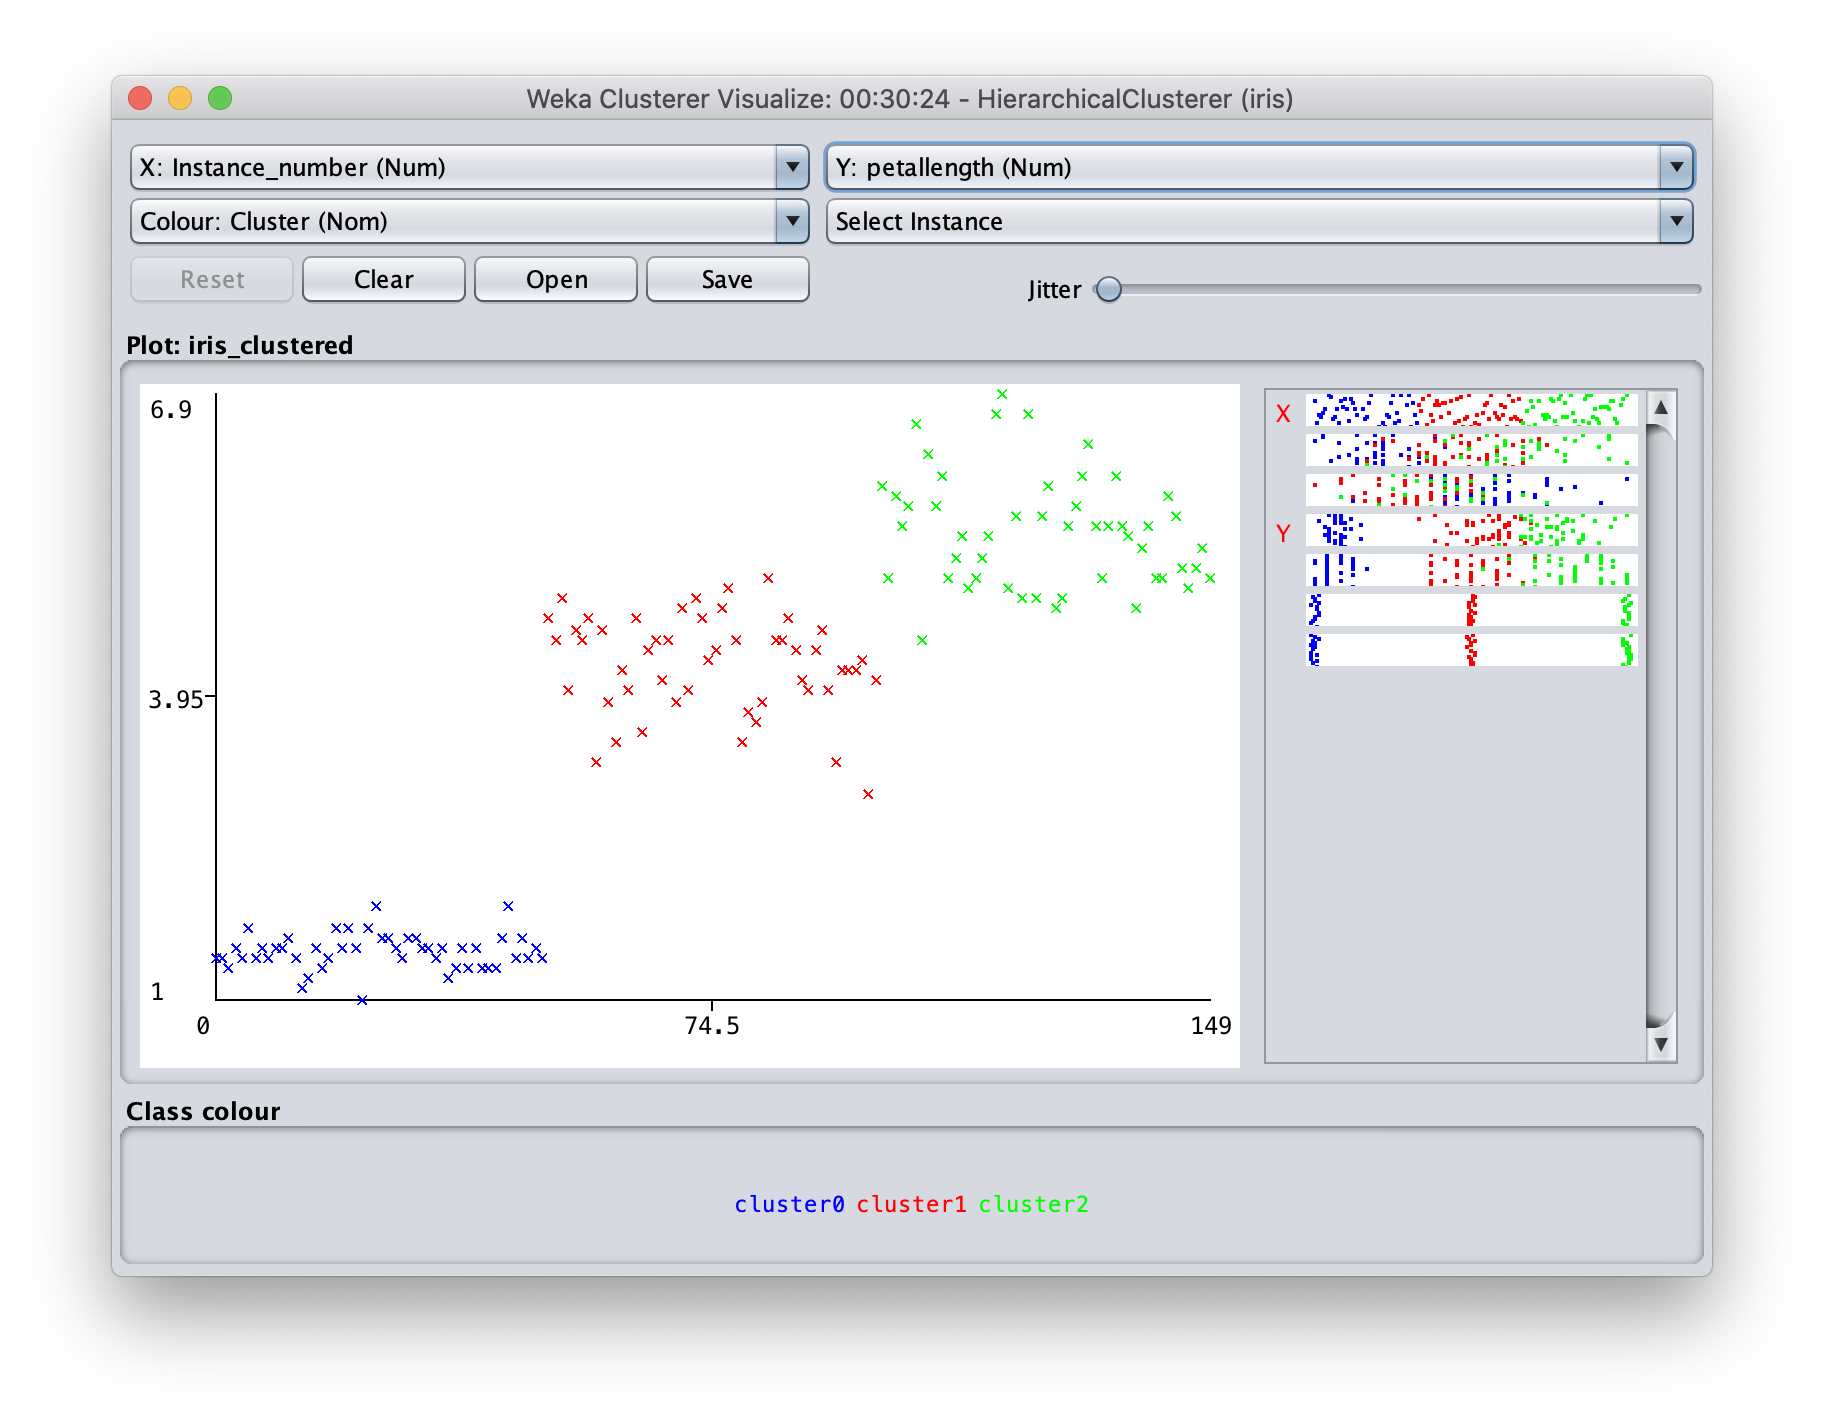
\includegraphics[scale=0.5]{hc_petallenght.png}
	\caption{X instance\_number con distancia Manhattan.}
	\label{Captura_5}
\end{figure}

\begin{figure}[h]
	\centering
	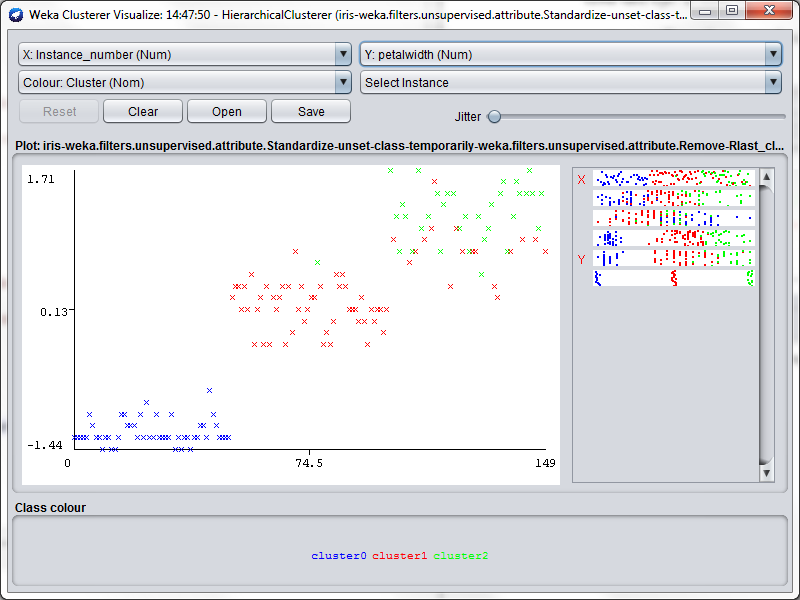
\includegraphics[scale=0.5]{hc_petalwidth.png}
	\caption{X instance\_number con distancia Manhattan.}
	\label{Captura_6}
\end{figure}


\begin{figure}[h]
	\centering
	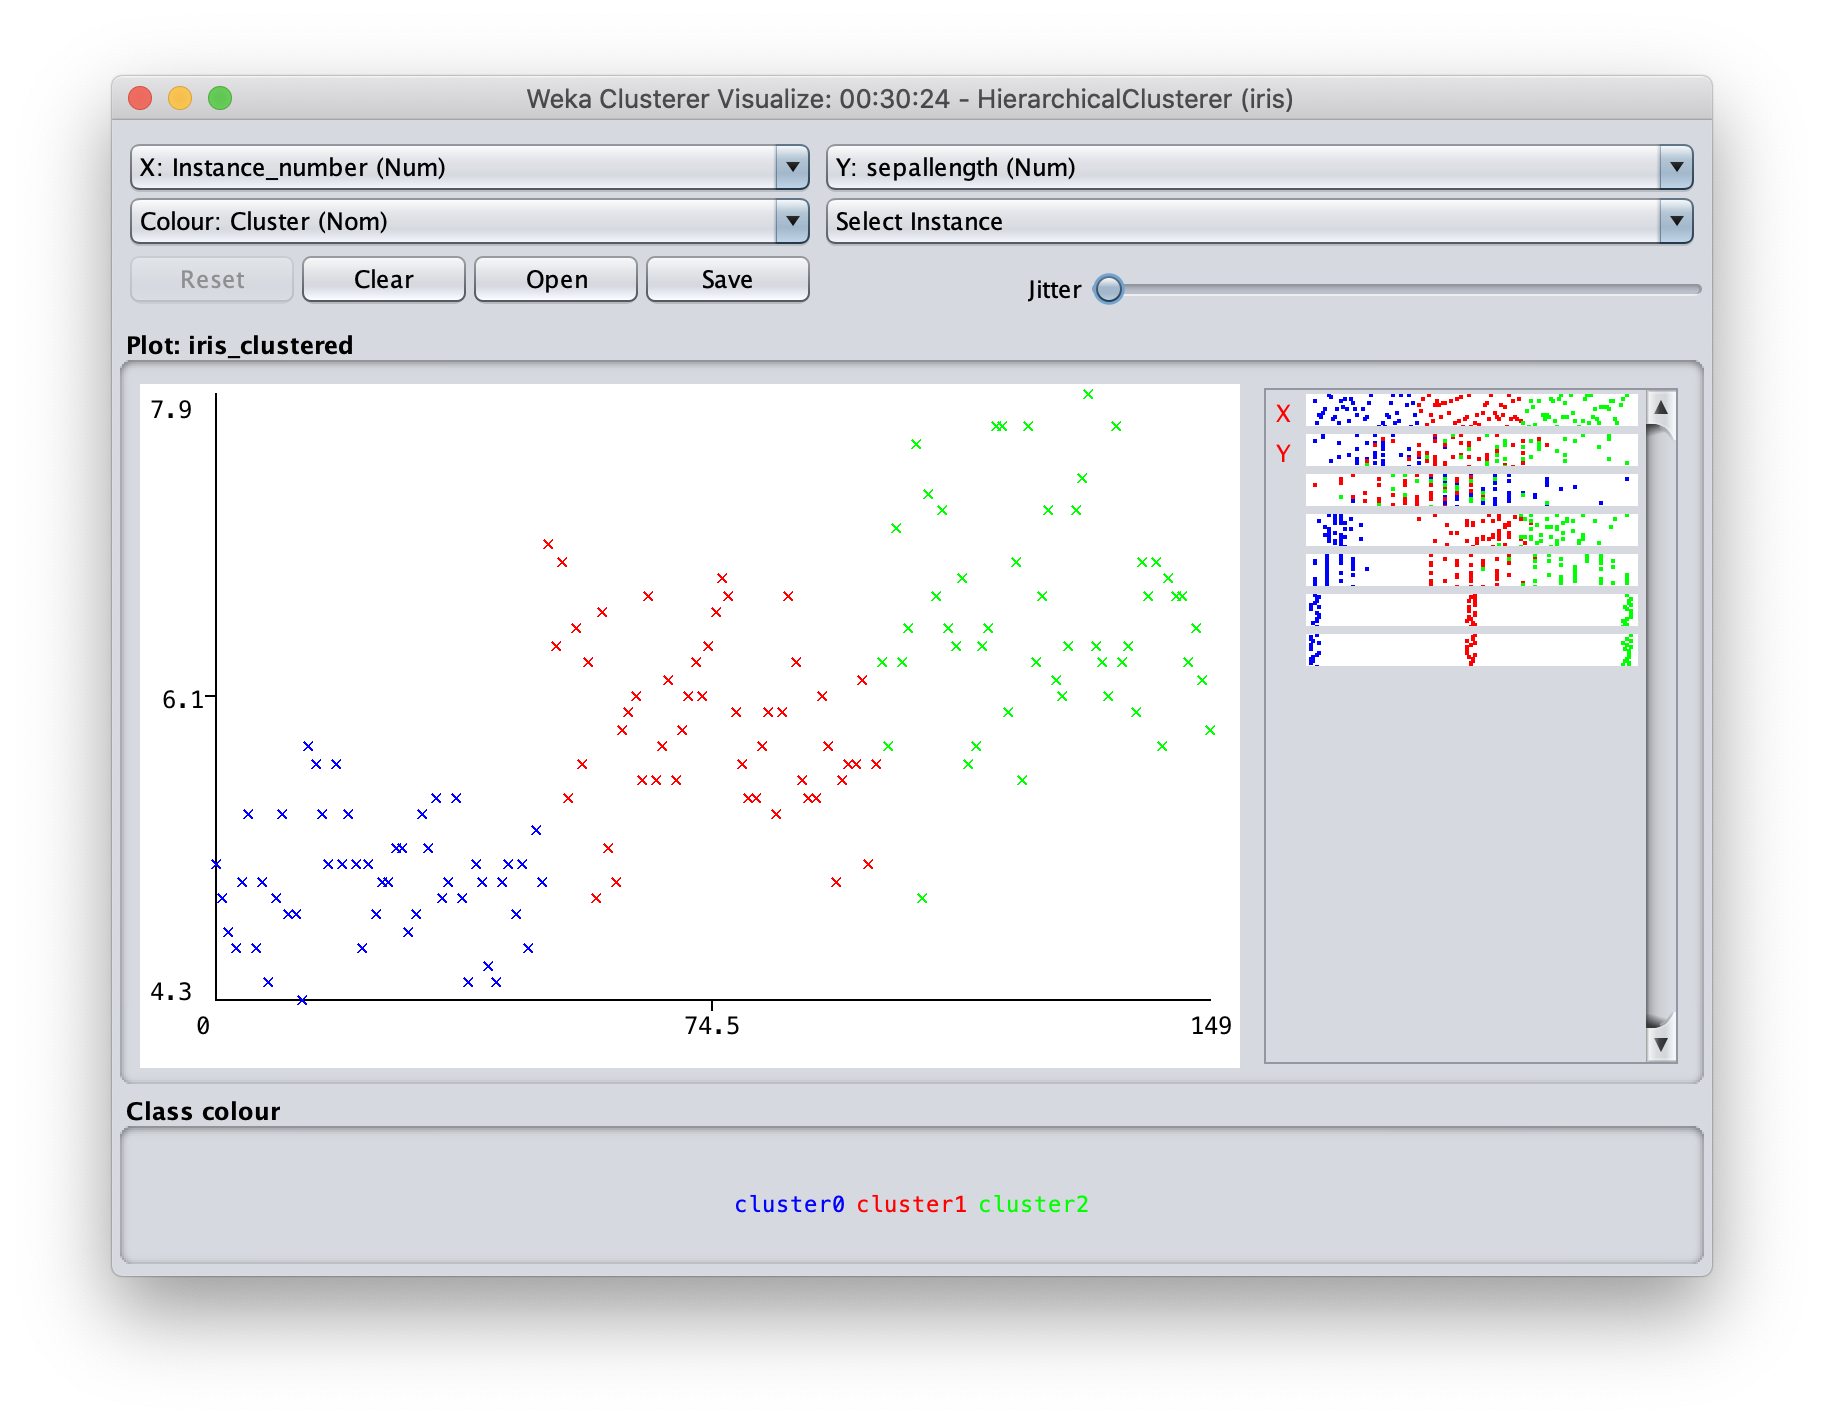
\includegraphics[scale=0.5]{hc_sepallebgth.png}
	\caption{X instance\_number con distancia Manhattan.}
	\label{Captura_7}
\end{figure}


\begin{figure}[h]
	\centering
	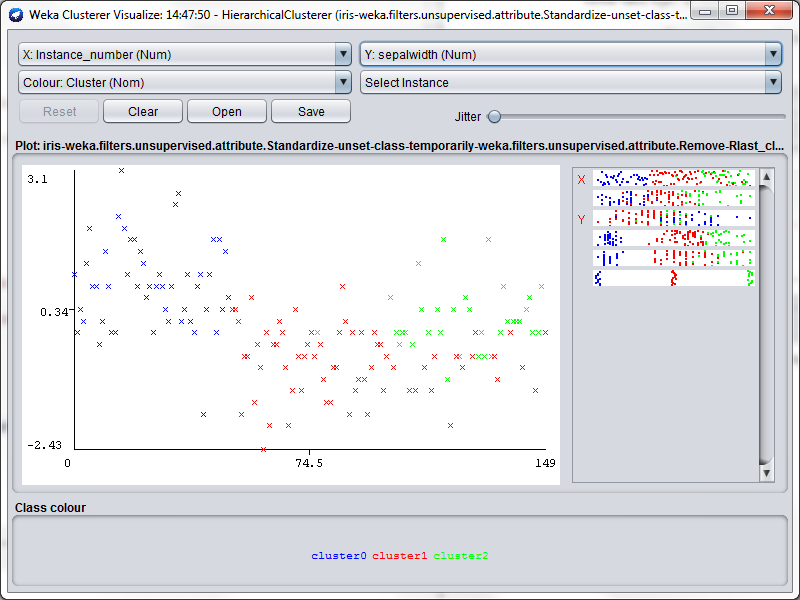
\includegraphics[scale=0.5]{hc_sepalwidth.png}
	\caption{X instance\_number con distancia Manhattan.}
	\label{Captura_8}
\end{figure}

\begin{figure}[h]
	\centering
	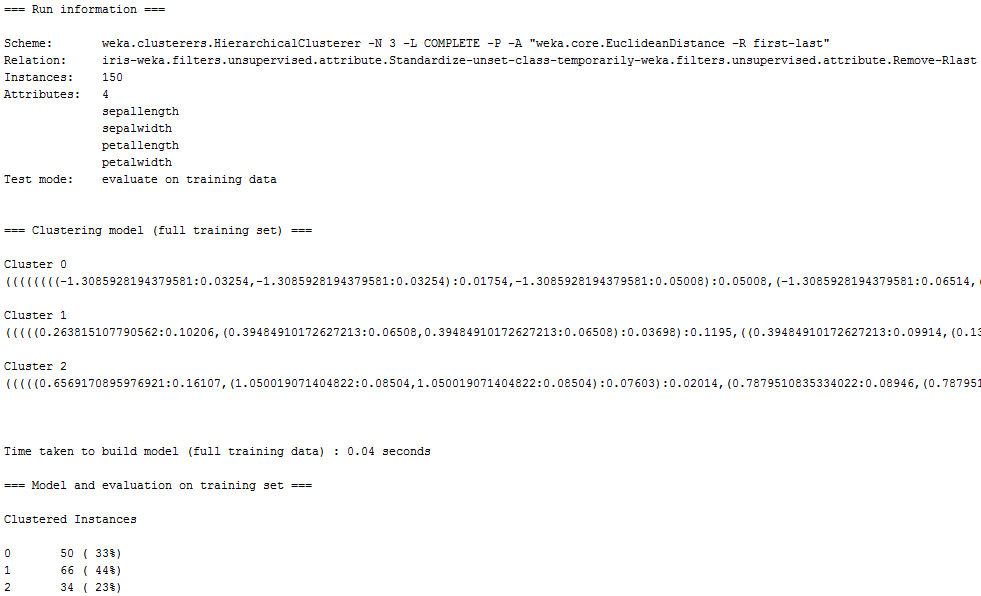
\includegraphics[scale=0.5]{hc_euclidea.png}
	\caption{Hierarchical Clustering con distancia Euclídea.}
	\label{Captura_9}
\end{figure}

\end{questions}

\end{document}
